\documentclass[12pt]{article}

\usepackage{sbc-template}

\usepackage{graphicx,url}

\usepackage[brazil]{babel}   
%\usepackage[latin1]{inputenc} 
% suporte para utf8
\usepackage[utf8]{inputenc}
\usepackage{aeguill} 

     
\sloppy

\title{Implementação de um Simulador para Processador RISC com Pipeline}

\author{Gabriel Araújo de Souza\inst{1}, Jaine Rannow Budke\inst{2}, Mayra Dantas de Azevedo\inst{3} }


\address{Instituto Metrópole Digital -- Universidade Federal do Rio Grande do Norte
  (UFRN)\\
  Caixa Postal 1524 -- 59.078-970 -- Natal -- RN -- Brazil
  \email{gabrieljucurutu@gmail.com, jainebudke@hotmail.com,
  mayradazevedo@gmail.com}
}

\begin{document} 

\maketitle

\section{Introdução}
O presente trabalho consiste na implementação de uma arquitetura para um conjunto de instruções (ISA, Instruction-Set Architecture) composta por Parte de Controle e Parte Operativa, compatíveis com a filosofia RISC (Reduced Instruction-Set Computer) e que executam em pipeline um conjunto de instruções. A simulação da arquitetura foi implementada na linguagem de propósito geral, Java.

O projeto foi desenvolvido levando em consideração conceitos aprendidos ao longo da disciplina Organização e Arquitetura de Computadores (OAC). Assim, foi utilizada da compreensão de processadores RISC e suas filosofias, o funcionamento de processadores visando a execução de microinstruções referentes a Instruções mais complexas entendidas pelo hardware, funcionamento de hardware e suas comunicações entre componentes, utilização de pipeline e suas melhorias no desempenho na execução de sequências de instruções, entre outros.

Este relatório tem como objetivo apresentar o planejamento do projeto, as principais decisões tomadas, os resultados obtidos e discutir acerca dos problemas encontrados a partir da organização definida, bem como futuras implementações que podem ser feitas como melhorias da solução.

A construção de problemas como esse contribui para o entendimento sobre elementos básicos de implementações em hardware, como por exemplo os conceitos de porta, sinal e canal, bem como para a fixação dos conhecimentos sobre o projeto e funcionamento dos processadores utilizados no mundo real.

\section{Decisões de Projeto}

\subsection{Tamanho da palavra do processador}

O endereçamento do processador MIPS é feito com palavras de 4 bytes (32 bits). Deste modo, tomando esta característica como base, utilizaremos para o projeto palavras de 32 bits.

\subsection{O formato da palavra de instrução}

O formato de instrução a ser usado será do tipo R, e segue a seguinte estrutura:
$$op \ rt \ rd \ rs \ shamt$$
Sendo:

\setlength{\parindent}{0cm}
$\bullet$ op: opcode (operação básica da instrução)\\
$\bullet$ rt: registrador destino\\
$\bullet$ rd: primeiro registrador fonte\\
$\bullet$ rs: segundo registrador fonte\\
$\bullet$ shamt: "shift amount" (para instruções de deslocamento)

\subsection{Os modos de endereçamento de operandos}
Foi considerado dois modos de endereçamento dos operandos como válidos:

$\bullet$ Imediato;\\
$\bullet$ Registrador.

\setlength{\parindent}{1.5cm}
O modo imediato é equivalente à ação de quando se tenta acessar uma instrução passando diretamente o endereço. 
Por exemplo:
$$lw \ R4, \ \$3, \ 0, \ 0$$

Nesse tipo de instrução é carregado diretamentamente da memória, um dado armazenado na posição 3 de memória e salvo no registrador de índice 4 do banco de registradores.

O modo registrador corresponde às instruções a serem executadas por meio da recuperação dos valores armazenados anteriormente nos registradores.
Por exemplo:
$$add \ R4, \ R3, \ R2, \ 0$$

Nessa instrução, primeiro é recuperado valores armazenados nos registradores fonte (índices 3 e 4 do banco de registradores), executado uma soma entre eles e o resultado da operação é salvo no registrador destino, que neste caso é o registrador de índice 4.

\subsection{O tamanho do banco de registradores}
O banco de registradores do MIPS é composto por 32 registradores. Assim, optamos por manter essa quantidade.

\subsection{O tamanho das memórias de instruções e de dados}
As instruções e os dados são guardados em vetores com 1000 posições de memória. Cada posição armazena uma palavra de 32 bits (definido em A).

\subsection{O número e tipos de barramentos da parte operativa}
A arquitetura foi implementada com barramentos dedicados entre os componentes que interagem entre si.

\section{Descrição da Solução}

O projeto foi implementado tendo como requisito explorar a abstração do funcionamento em hardware. Desta forma, inicialmente foram implementadas as classes Signal, Port e Canal, com o propósito de simular como ocorre a conexão entre componentes físicos. Além disso, foram criadas classes para os componentes que compõem uma arquitetura básica de processamento: a Unidade Lógica e Aritmética (ULA), Memória de Dados, Memória de Instruções, Decodificador, Contador de Programa, Registrador e o Banco de Registradores.

    Na implementação de um componente de hardware é considerado que ele possui portas de entrada e saída, um componente é ligado a outro por meio de canais, um canal conecta uma porta de saída de um componente a uma porta de entrada de outro, os dados das execuções realizadas por um componente são entendidas através de sinais, um sinal sai por uma porta de saída e fica em um canal até que seja lido, quando um componente deseja receber algum dado, a porta de entrada dele recebe o dado que está escrito no canal que a conecta e o libera, um canal que possui um dado escrito não pode receber outro enquanto esse não for consumido. 

A arquitetura foi implementada com barramentos dedicados, em que todos os componentes conectam-se diretamente e os dados são escritos e acessados diretamente dos canais. A implementação ocorreu de forma que inicialmente, todos os canais são criados, para então realizar a conexão entre os componentes através de suas portas. Em seguida, as memórias de instruções e de dados são carregadas com suas respectivas informações. A partir deste ponto, os componentes estão prontos para terem suas portas checadas e serem executados.

O Contador de Programa (PC) busca a próxima instrução a ser lida e envia um sinal para a porta de saída, que está conectada, por meio de um canal, com a porta de entrada da Memória de Instruções. Dessa forma, o segundo componente tem em sua entrada a próxima instrução a ser lida.

Em seguida, a Memória de Instruções recupera a instrução atual e escreve no canal que se comunica com o grupo de registradores para realizar a leitura dos operandos. O Banco de Registradores, então, recupera a instrução, a decodifica (por meio do Decoder) e a interpreta de acordo com o esperado. Assim, o banco de registradores passa a ser o responsável por fazer o intermédio com o Decodificador de Instruções, bem como possui sinal de acesso direto à Memória de Dados, ele é formado por 32 registradores, responsáveis pelo armazenamento de resultados/dados temporários ou que são buscados/recuperados da Memória de Dados.

O Decoder intermediado pelo Banco de Registradores é o responsável por decodificar a instrução recebida de acordo com o formato pré-estabelecido (nas decisões de projeto), identificando o opcode, os registradores fonte e destino, bem como se há um salto de instrução. Além disso, o Decoder é quem especifica e faz as chamadas particulares de cada uma das diferentes instruções.

Neste contexto, o Decoder foi implementado de modo que seja capaz de interpretar e executar corretamente as seguintes instruções:

\subsection{AND, OR, XOR, NOT}
Quando o Decoder identifica uma dessas operações, é estabelecida uma comunicação com a ULA, a qual efetua a operação e escreve no canal que está conectado com o Banco de Registradores, que transfere o resultado para o registrador especificado.

\subsection{ADD}
Quando é detectado o opcode ADD, a arquitetura identifica os registradores fonte e o registrador destino e os operandos são gravados no canal que se comunica com o componente ULA, o qual é responsável por executar a operação de adição e retornar o resultado para o Banco de Registradores.

\subsection{SUB}
O opcode SUB é semelhante ao ADD. Os registradores fonte e destino são detectados e a ULA fica responsável pela operação de subtração e por retornar o resultado ao Banco de Registradores.

\subsection{LW}
A instrução com o opcode LW assume a responsabilidade de carregar um dado da memória de dados em algum registrador do banco de registradores. Então, quando LW é detectado, o Decoder identifica o endereço de memória no qual o dado será buscado e o registrador que irá armazenar temporariamente o dado. Após a identificação, o endereço é salvo no canal por meio de um sinal que se comunica com a porta de entrada da memória de dados, a qual busca o dado localizado no endereço especificado e o escreve na porta de entrada do Banco de Registradores que, por sua vez, atualiza o registrador destino com o dado recebido.

\subsection{ST}
A instrução ST tem a função de transferir um dado de um registrador para a memória de dados. Desta forma, quando o opcode é reconhecido, o decoder identifica o registrador fonte e o endereço de memória ao qual o dado será destinado. Após isso, o dado e o endereço especificado são escritos na porta de entrada da Memória de Dados que, ao detectar um sinal, grava o dado no endereço descrito.

A unidade lógica e aritmética (ULA) recebe um sinal de controle. A partir desse sinal, o decodificador que a ULA possui é o responsável por definir qual a operação deve ser executada. Após a execução, o resultado é escrito no canal que mantém a comunicação entre a ULA e o banco de registradores, de modo que a resposta possa ser gravada no registrador destino da instrução aritmética. A unidade lógica tem ainda uma saída de apenas 1 bit, que possui valor equivalente a verdadeiro se a operação resulta em zero e falso caso contrário.

A Memória de Dados é o componente responsável por ler os dados disponíveis na memória e disponibilizá-los para os demais componentes. Sua execução consiste em ler as portas de entrada para recuperar os dados que devem ser gravados ou recuperados na memória. No caso de dados que devem ser lidos da memória, ainda é necessário enviar essas informações para o banco de registradores através do canal que liga a saída da Memória de Dados à entrada do Banco de Registradores.

    É possível visualizar as conexões entre os componentes citados no diagrama de blocos da parte operativa que se encontra abaixo:

\begin{figure}[!ht]
\centering
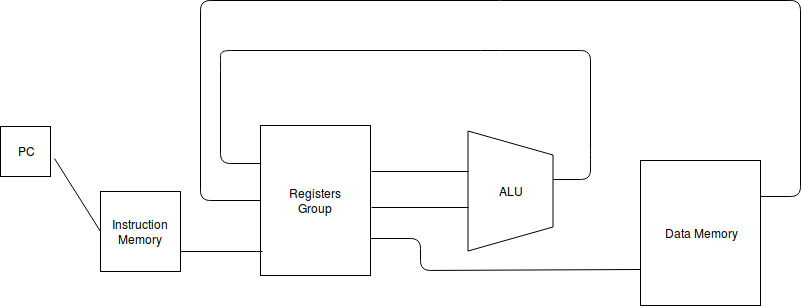
\includegraphics[width=.9\textwidth]{img/op1.jpeg}
\caption{Diagrama de blocos da parte Operativa}
\label{fig:blocosOperativa}
\end{figure}

\begin{figure}[!ht]
\centering
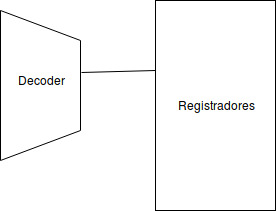
\includegraphics[width=.4\textwidth]{img/op2.jpeg}
\caption{Componentes do Banco de Registradores}
\label{fig:blocosOp2}
\end{figure}

\section{Pipeline}
O pipeline é uma metodologia de melhoria de desempenho que consiste em reaproveitar componentes ociosos durante o processo de execução. Com ele, microinstruções de instruções diferentes podem executar em paralelo, assim, em determinado momento, o processador terminará de executar uma instrução por ciclo de relógio, quando isso ocorre, diz-se que o pipeline está cheio. Ele é dividido em pequenos grupos chamados de estágios, cada estágio é responsável por executar uma microinstrução diferente, portanto, quando é decidido a implementação de um pipeline, deve-se também dividir cada instrução reconhecida pelo processador em um grupo de microinstruções iguais, permitindo assim o uso da metodologia.

    Para este projeto, foi decidido implementar um pipeline de 5 estágios, são esses: carregamento da instrução, decodificação da instrução, leitura dos operandos fonte, execução das operações e armazenamento dos resultados obtidos. Caso fosse desejado um pipeline de 4 estágios, por exemplo, deveria dividir as instruções em 4 microinstruções e organizá-las de forma a evitar conflitos decorridos dessas mudanças, uma sugestão seria juntar a decodificação da instrução e a leitura dos operandos fontes em um único estágio de pipeline, permanecendo inalterados os demais. 

A parte de controle do processador é composta por um while que é responsável por executar cada microinstrução em uma sequência de execuções em paralelo utilizando o pipeline, como exemplo da coordenação dessas ações será mostrado a seguir o diagrama de controle para a seguinte sequência de instruções:

$$
lw \ R1 \ \$1 \ 0 \ 0; $$$$
lw \ R2 \ \$2 \ 0 \ 0; \\$$$$
lw \ R4 \ \$3 \ 0 \ 0; \\$$$$
lw \ R5 \ \$4 \ 0 \ 0; \\$$$$
lw \ R6 \ \$5 \ 0 \ 0; \\$$$$
add \ R3 \ R1 \ R2 \ 0; \\$$$$
sub \ R7 \ R5 \ R4 \ 0; \\$$$$
st \ \$6 \ R3 \ 0 \ 0;$$
$$$$

O controle para a execução dessas operações pode ser vista na Figura~\ref{fig:operativa}

\begin{figure}[h]
\centering
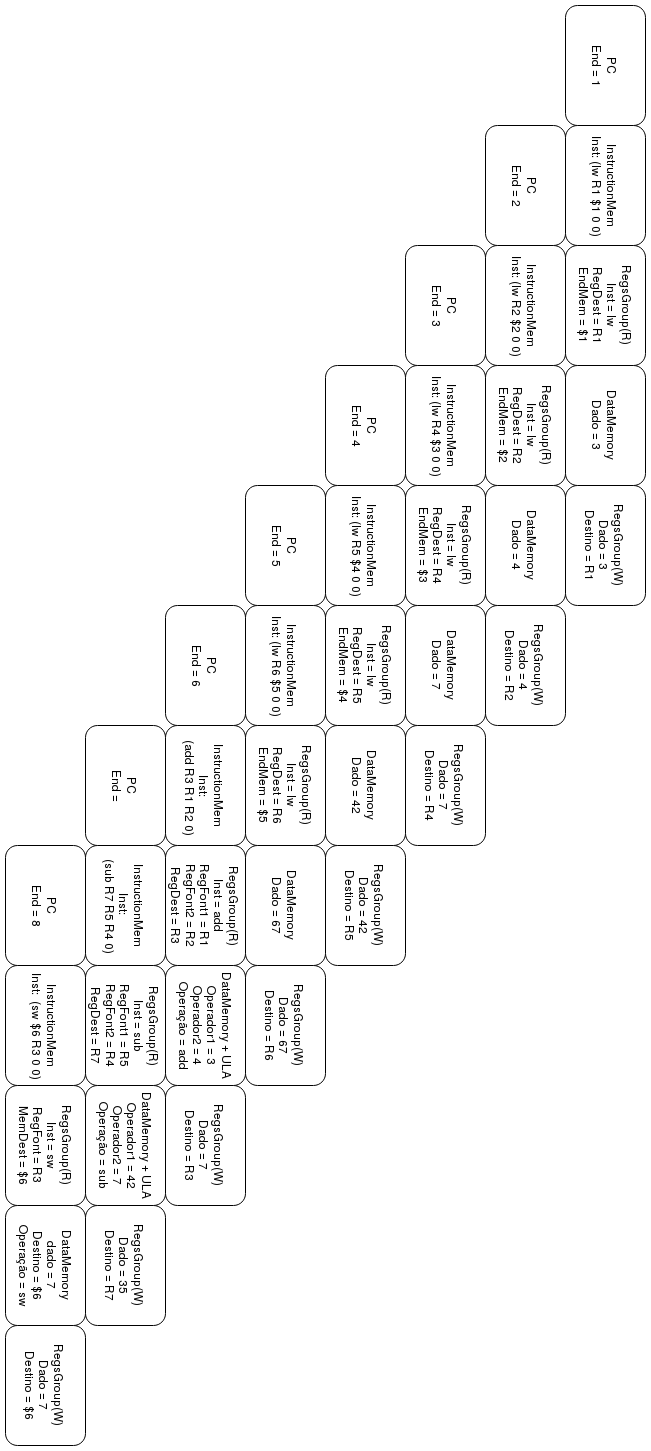
\includegraphics[width=.7\textwidth]{img/diagramaControle.png}
\caption{Diagrama da parte Operativa - Execução com Pipeline}
\label{fig:operativa}
\end{figure}

Por meio do diagrama é facilmente notável o preenchimento dos estágios do pipeline, para a execução dessas 8 instruções são necessários 11 ciclos de relógio, caso não houvesse o uso do pipeline e cada microinstrução dessa fosse executado em um ciclo único de relógio, seria necessário 40 ciclos, mesmo que um ciclo individual execute em um período de tempo menor ao de cada estágio, ainda assim haveria ganho em relação ao uso de pipeline, sabendo disso é notório a melhoria do desempenho ao se utilizar de tal metodologia.

Uma observação importante é que a sequência de instruções foi cuidadosamente selecionada para evitar erros durante a execução, como por exemplo, conflitos de dados, este ocorre quando uma instrução necessita de um dado que outra instrução ainda não armazenou no local em comum. O sistema desenvolvido não é capaz de lidar com problemas desse tipo, para tanto, é importante que o programador que use esse sistema tenha o cuidado de evitar dependências de dados ou de controle entre os estágios de execução. Algumas medidas que podem ser tomadas para amenizar os problemas como a inserção de instruções antes de uma que dependa de dados de outra instrução, utilização dos demais registradores para evitar a dependência ou a sobrescrita de um dado, utilizar-se dos modos de endereçamento oferecidos pelo simulador, dentre outras medidas.

As instruções de saltos também não puderam ser implementadas, embora o grupo tenha debatido a forma como cada uma deveria ser implementada. Mesmo sabendo o que poderia ser feito, foi optado por deixar tais modificações como possíveis melhorias futuras para o simulador, levando em consideração que deveria ser feito algumas alterações significativas na lógica de controle implementada.

\section{Conclusão}

Diante do desafio de implementar um simulador de um processador RISC em uma linguagem de programação que não utiliza, por padrão, os conceitos de hardware, o grupo pôde ter uma experiência proveitosa ao ter que implementar conceitos como o de componente, sinal, canal e porta. Durante a implementação destes, obteve-se uma melhor compreensão do funcionamento de um componente, a necessidade de manter tais conceitos durante toda implementação, fez com se visse na prática os diversos estudos realizado durante o semestre na disciplina.

Para tanto, vê-se a importância de elaborar tais metodologias em sala de aula. O aluno, assim, consegue associar melhor aquilo que é visto quando se sente na necessidade de aplicar os conhecimentos obtidos em algo na vida real. A elaboração do simulador foi um meio de forte aprendizado. A inserção de trabalhos como estes, estimula o aluno a sempre buscar mais sobre conteúdos teóricos visto na universidade, na área de Tecnologia da Informação, atividades como estas, garante uma boa formação e preparação para graduandos.

Embora não tenha sido possível implementar todas as características necessárias da metodologia pipeline em processadores RISC, houve a discussão entre o grupo de como os atributos faltosos poderiam ser implementados. Este tipo de análise sobre o que foi feito e o que poderia ter sido melhorado, contribui para a reflexão do aluno em meio aos seus trabalhos produzidos, uma forma saudável de autoavaliação, como também a interação e divisão de tarefas em um grupo.

Além disso, o componente Decoder dá suporte, também, às instruções de comparação (CMP), salto incondicional (J), Salto Condicional - salta se Negativo (JN) e Salto Condicional - salta se Zero (JZ). Contudo, a implementação lógica adicional de cada uma delas não foi especificada na codificação, de modo que não é feita a chamada de componentes auxiliares que compõem a finalização da execução.

\end{document}
